\documentclass[11pt,a4paper,twoside]{article}
\usepackage[utf8]{inputenc}
\usepackage{fullpage}
\usepackage[english]{babel}
%\usepackage{times}

\usepackage{hyperref}

\usepackage{vmargin}
%\setmarginsrb{a}{b}{c}{d}{e}{f}{g}{h} 
% a la marge de gauche
% b la marge haute
% c la marge de droite
% d la marge basse
% e la hauteur de l'en-tête
% f la distance entre l'en-tête et le texte
% g la hauteur du pied-de-page
% h la hauteur totale entre le bas de page et le bas du pied de page
\setpapersize{A4}
%\setmarginsrb{1.5cm}{1.5cm}{1.5cm}{1.5cm}{0cm}{0cm}{0cm}{0cm}
\setmarginsrb{1.5cm}{1.5cm}{1.6cm}{1.5cm}{0.4cm}{0.3cm}{0.4cm}{0.8cm}
\renewcommand{\baselinestretch}{.97}
%%%%%%%%% header/footer format %%%%%%%%%%%%%
% NOTE: Copy from D2.1.1 deliverable.
\usepackage{lastpage}
\usepackage{fancyhdr}
\usepackage{isodayandtime}
%\usepackage{asmmath}
%%%%%%%%% header/footer format %%%%%%%%%%%%%
\pagestyle{fancy}
\fancyhead{}
\fancyhead[RO]{\sffamily \small The Discovery Initiative, DIstributed and COoperative management of Virtual Environments autonomouslY}
\fancyhead[C]{}
\fancyhead[LE]{\sffamily \small Beyond the Clouds, How Should Next Utilty Computing Infrastructures Be Designed}
\fancyfoot[RO,LE]{}
%\fancyfoot[C]{\thepage/\pageref{LastPage}}
\fancyfoot[C]{\thepage/\pageref{LastPage}}
\fancyfoot[LO,RE]{}
\renewcommand{\headrulewidth}{.1pt}

\def\myog{{\rm~\og{}}}\def\myfg{{\rm\fg{}~}}

\fancypagestyle{plain}{% follow n/m page number format on plain pages too
\fancyhead[RO,LE]{}
\fancyhead[RO,LE]{\sffamily \small DIstributed and COoperative management of Virtual Environments autonomouslY}
\fancyhead[C]{}
\fancyhead[LO,RE]{}
   \fancyfoot[C]{}
}
%%%%%%%%%%%%%%%%%%%%%%%%%%%%%%%%%%%%%%%%%%%%
\usepackage{xspace}
\newcommand{\discovery}{DISCOVERY\xspace}
\newcommand{\ie}{\textit{i.e.}\xspace}
\usepackage[textwidth=17mm]{todonotes}

\usepackage{ifthen}
\newboolean{WIP}
\gdef\ifwip{\ifthenelse{\boolean{WIP}}}
\setboolean{WIP}{false}%
%\setboolean{WIP}{true}%
\ifwip{
  %% TODOs for WP leaders
  \newcommand{\indication}[1]{{\it\color{red}#1}\\}
  \newcommand{\AL}[2][inline]{\todo[color=green!50,#1]{\sf \textbf{AL:} #2}} 
  \newcommand{\PA}[2][inline]{\todo[color=blue!20,#1]{\sf \textbf{PA:} #2}} 
  \newcommand{\ER}[2][inline]{\todo[color=yellow!50,#1]{\sf \textbf{ER:} #2}} 
  \newcommand{\RN}[2][inline]{\todo[color=brown!50,#1]{\sf \textbf{RN:} #2}} 
  \newcommand{\TC}[2][inline]{\todo[color=orange!50,#1]{\sf \textbf{TC:} #2}} 
  \newcommand{\TR}[2][inline]{\todo[color=purple!60,#1]{\sf \textbf{TR:} #2}} 
  \newcommand{\TODO}[2][inline]{\todo[color=red!50,#1]{\sf #2}} 

	\newcommand{\ALinst}{Mines Nantes\xspace}  % Mines Nantes
	\newcommand{\RNinst}{BSC\xspace}  % BSC
	\newcommand{\PAinst}{CRS4\xspace}  % CRS4
	\newcommand{\TRinst}{EPFL\xspace}  % EPFL
	\newcommand{\ETinst}{Neuchatel\xspace} % Neuchatel
}{
  \newcommand{\indication}[1]{}
  \newcommand{\AL}[2][]{}
  \newcommand{\PA}[2][]{}
  \newcommand{\ER}[2][]{}
  \newcommand{\RN}[2][]{}
  \newcommand{\TC}[2][]{}
  \newcommand{\TR}[2][]{}
  \newcommand{\TODO}[2][]{}

	\newcommand{\ALinst}{partner~1\xspace}  % Mines Nantes
	\newcommand{\RNinst}{partner~2\xspace}  % BSC
	\newcommand{\PAinst}{partner~3\xspace}  % CRS4
	\newcommand{\TRinst}{partner~4\xspace}  % EPFL
	\newcommand{\ETinst}{partner~5\xspace} % Neuchatel

}

\usepackage{color,colortbl}
\usepackage{xcolor}
\usepackage{multirow}
\usepackage{array}
\usepackage{xtab}
\usepackage{wrapfig}

%\title{Beyond the Clouds\\ 
%\vspace*{.6cm}the DISCOVERY Initiative}
\begin{document}

%% Begining of the first page

\sffamily
\thispagestyle{empty}
\begin{center}
%{\large \textbf{Small or medium-scale focused research project (STREP)}}\\
{\large \textbf{}}\\
\vspace*{.5cm} 
\large{\textbf{Fact Sheet}}\\
\vspace*{.5cm} 
%\large{\textbf{ICT FET Open Call}\\FP7-ICT-2011-C}\\
%\AL{FET Open or Young Researcher, Mathieu ?}
%\vspace*{1cm}
{\LARGE Beyond the Clouds, How Should Next\\ Utility Computing Infrastructures Be Designed?}\\~\\
{\LARGE \textbf{The DISCOVERY Initiative}\\~\\
{\LARGE DIstributed and COoperative management of Virtual Environments autonomouslY}}\\
%\vspace*{1cm}
%{\LARGE\textbf{DISCOVERY}}
\end{center}

\begin{center}
\large{\textbf{Date of preparation: \today}}\\
\large{Version:~\isodayandtime}
\end{center}

%\vspace*{.5cm}
%\noindent\large{Type of funding scheme: Small or medium-scale focused research project (STREP), short proposal}\\
%\large{\textbf{Work program topics addressed: ICT-2011.9.3 FET Young Explorers}}\\

\vspace*{2cm}
\noindent \textbf{\large{Proposal Abstract:}}\\

\vspace*{.1cm}
\noindent\parbox{1\textwidth}{
The DISCOVERY initiative aims at exploring a new way of operating Utility Computing (UC) resources. 

\medskip
To accommodate the ever-increasing demand for Utility Computing (UC) resources, while taking
into account both energy and economical issues, the current trend consists in
building larger and larger data centers in a few strategic locations. Although
such an approach enables to cope with the actual demand 
while continuing to operate UC resources through centralized
software system, it is far from delivering sustainable and efficient UC infrastructures. 
%
We claim that a disruptive change in UC infrastructures is required: UC
resources should be managed differently, considering locality as a
primary concern. To this aim, \textbf{we propose to leverage any facilities available through the
Internet in order to deliver widely distributed UC platforms that can better
match the geographical dispersal of users as well as the unending demand.
Critical to the emergence of such locality-based UC (LUC) platforms is
the availability of appropriate operating mechanisms. We
advocate the implementation of a unified system driving the use of
resources at an unprecedented scale by turning a complex and diverse
infrastructure into a collection of abstracted computing facilities that is
both easy to operate and reliable.} 

\medskip
By deploying and using such a \emph{LUC Operating System} on backbones,
our ultimate vision is to make possible to host/operate a large part of the
Internet by its internal structure itself: A scalable and nearly infinite set
of resources delivered by any computing facilities forming the Internet,
starting from the larger hubs operated by ISPs, government and academic
institutions to any idle resources that may be provided by end-users. 
%
Unlike previous researches on distributed operating systems, we propose to
consider virtual machines (VMs) instead of processes as the basic element.  System
virtualization offers several capabilities that increase the flexibility of
resources management, allowing to investigate novel decentralized schemes that
will enable to achieve the LUC infrastructure we target.
} 
%\pagebreak

%\textbf{IPL-DISCOVERY}

\bigskip
\noindent
\textbf{Consortium:}

\textbf{Coordinator} - Adrien L{\`e}bre (Mines de Nantes, Inria Rennes Bretagne Atlantique, adrien.lebre@inria.fr)

\textbf{Inria}(Asap, Ascola, Avalon, Myriads - France),  Orange R\&D (France), Renater (France), BSC (Spain), CRS4(Italy), PSNC (Poland), GRNET (Greece)



\smallskip
\noindent \textbf{Web site:} \url{http://beyondtheclouds.github.io}

\smallskip
\noindent\textbf{Contributors:} Marin Bertier, Thierry Coupaye, Fr{\'e}d{\'e}ric Desprez, Adrien Lebre, Anne-Cécile Orgerie, Jonathan Rouzaud-Cornabas, Cédric Tedeschi.
%% End of the first page
\pagebreak

\thispagestyle{fancy} 
\setcounter{page}{1}
%\thispagestyle{empty}
%\setmarginsrb{2.5cm}{2cm}{2.5cm}{2cm}{0cm}{0.2cm}{0cm}{0.2cm}

\section{Context\label{sec:intro}}

%% Motivation 
\subsection{Current Trends.}

The success of Cloud Computing has driven the advent of Utility Computing~(UC). However, Cloud
Computing is a victim of its own success: In order to answer the escalating demand for
computing resources, Cloud Computing providers must build data centers~(DCs) of
ever-increasing size. As a consequence, besides facing the well-known issues of large-scale platforms
management, large-scale DCs have now to deal with energy considerations that limit the number
of physical resources that one location can host.

Instead of investigating alternative solutions that could tackle the aforementioned
concerns, the current trend consists in deploying larger and larger DCs in few strategic
locations presenting energy advantages. For example, Western North Carolina, USA, is an
attractive area due to its abundant capacity of coal and nuclear power brought about the
departure of the textile and furniture industry~\cite{greenpeace:2013}. More recently,
several proposals suggested building next generation DCs close to the polar circle in
order to leverage free cooling techniques, considering that cooling is accounting for a
big part of the electricity consumption~\cite{greenberg:sigcomm09}.

%%%
\subsection{Inherent Limitations of Large-scale DCs}

Although building large scale DCs  enables to cope with the actual demand,
% while continuing to operate UC resources through centralized software system 
it is far from delivering sustainable and efficient UC infrastructures. In addition to
requiring the construction and the deployment of a complete network infrastructure to
reach each DC, it exacerbates the inherent limitations of the Cloud Computing model:

\begin{itemize}
\item The externalization of private applications/data often faces legal issues that
  restrain companies from outsourcing them on external infrastructures, especially when
  located in other countries.
\item The overhead implied by the unavoidable use of the Internet to reach distant
  platforms is wasteful and costly in several situations: Deploying a broadcasting service
  of local events or an online service to order pizzas at the edge of the polar circle,
  for instance, leads to important overheads since most of the users are \emph{a priori}
  located in the neighborhood of the event/the pizzeria.
\item The connectivity to the application/data cannot be ensured by centralized dedicated
  centers, especially if they are located in a similar geographical zone. The only way to
  ensure disaster recovery is to leverage distinct sites.\footnote{``Amazon outages –
    lessons learned'',
    \href{http://gigaom.com/cloud/amazon-outages-lessons-learned/}{http://gigaom.com/cloud/amazon-outages-lessons-learned/}
    (valid on Nov 2013, the 30\textsuperscript{th}).}
\end{itemize}

The two first points could be partially tackled by hybrid or federated Cloud
solutions~\cite{armbrust:2010}, that aim at extending the resources available on one Cloud
with those of another one; however, the third one requires a disruptive change in the way
UC resources are managed.
%Deploying a local events broadcasting service or an
%online service to order pizza at the edge of the polar circle for instance, leads to an important overhead
%in terms of energy footprint, network exchanges as well as latency since it can be assumed
%that a vast majority of the users are located in the neighborhood of the event/the
%pizzeria.

Another issue is that, according to some projections of a recent IEEE
report~\cite{ieeenetreport:2012}, the network traffic continues to double roughly every
year. Consequently, bringing the IT services closer to the end-users is becoming crucial
to limit the energy impact of these exchanges and to save the bandwidth of some
links. Similarly, this notion of locality is critical for the adoption of the UC
model by applications that need to deal with a large amount of data as getting them in and
out actual UC infrastructures may significantly impact the global
performance~\cite{Fos11}.

The concept of micro/nano DCs at the edge of the backbone~\cite{greenberg:sigcomm09} may
be seen as a complementary solution to hybrid platforms in order to reduce the overhead of
network exchanges. However, operating multiple small DCs breaks somehow the idea of
mutualization in terms of physical resources and administration simplicity, making this
approach questionable.
% Moreover, the number of such micro/nano DCs will remain limited and the question of
% where and how federating a large number of such facilities are still not solved.

%%%
\subsection{Ubiquitous and Oversized Network Backbones}

One way to partially solve the mutualization concern enlightened by the defenders of
large-scale DCs is to directly deploy the concept of micro/nano DCs upon the Internet
backbone. People are (and will be) more and more surrounded by computing resources,
especially those in charge of interconnecting all IT equipments. Even though these small
and medium-sized facilities include resources that are barely
used~\cite{Andrew:2003,Benson:2010}, they can hardly be removed (\textit{e.g.} routers).
Considering this important aspect, we claim that a new generation of UC platforms can be
delivered by leveraging existing network centers, starting from the core nodes of the
backbone to the different network access points in charge of interconnecting public and
private institutions. By such a mean, network and UC providers would be able to mutualize
resources that are mandatory to operate network/data centers while delivering widely
distributed UC platforms able to better match the geographical dispersal of users.
%
% TODO: AL -> ACO, please introduce this point latter in the chapter
% As a consequence, several initiatives started investigating how they could be
%better leveraged to support the requirements and constraints of current IT
%usages.  The concept of \emph{data furnaces} \cite{liu:hotcloud11} is one of
%the promising idea that seeks to mitigate the cost of operating
%network/computing resources by using them as a source of heat inside public
%buildings such as hospitals or universities. 
%
Figure~\ref{fig:renater} allows to better capture the advantages of such a proposal.
%\ftodo[FQ$\rightarrow$ALL]{Nous n'avons pas encore introduit la contribution à ce stade $\rightarrow$ enlever cette phrase~?}
% We did, cf. above : WE CLAIM
It shows a snapshot of the network weather map of
RENATER\footnote{\href{http://www.renater.fr}{http://www.renater.fr}}, the backbone
dedicated to universities and research institutes in France. It reveals several
important points:
\begin{figure}[htbp]
\vspace*{-.3cm}

\includegraphics[width=10cm]{./FIGS/renater.png}
\centering\caption{The RENATER Weather Map on May 2013, the 27th, around 4PM.
Each red square corresponds to a particular point of presence (PoP) of the network. The map is available in real-time
at: \href{http://www.renater.fr/raccourci}{http://www.renater.fr/raccourci}}
\label{fig:renater}
\vspace*{-.3cm}
\end{figure}



\begin{itemize} 
\item As mentioned before, most of the resources are underutilized (only two links are used
  between 45\% and 55\%, a few between 25\% and 40\%, and the majority below the threshold
  of 25\%).
\item The backbone was deployed and is renewed to match the demand: The density of points
  of presence~(PoP, \ie a small or medium-sized network center) as well as the bandwidth
  of each link are more important on the edge of large cities such as Paris, Lyon or
  Marseille.
\item The backbone was designed to avoid disconnections, since 95\% of the PoPs can be
  reached by at least two distinct routes.
\end{itemize}


%\ftodo[AL -> ALL]{It might make sense to talk of congestion effects that we can see in Marseille and Paris, the two path to the rest of Internet.}

\subsection{Locality-based Utility Computing}

Instead of building and deploying dedicated facilities, we claim that next UC
infrastructures should be tightly coupled with any facilities available through
the Internet, starting from the core routers of the backbone, the different
network access points and any small and medium-size computing infrastructures
that may be provisioned by public and private institutions. 
 Although it involves radical changes in the way
physical and virtual resources are managed, locating and operating computing and data on
facilities close to the end-users is the only way to deliver highly efficient
and sustainable UC services. 

From the physical point of view, network backbones 
%such as National Research and Educational Networks (NRENs) 
provide appropriate infrastructures, \ie, reliable and efficient enough to operate UC
resources spread across the different PoPs. Ideally, UC resources would be able to
directly take advantage of computation cycles available on network active devices,
\textit{i.e.} those in charge of routing packets. However, leveraging network resources to
make external computations may lead to important security concerns. Hence, we propose to
extend each PoP with a number of servers dedicated to hosting virtual machines~(VMs). Because it is natural
to assume that the network traffic and UC demands are proportional, larger network centers
will be completed by more UC resources than the smaller ones. Moreover, by deploying UC
services on relevant PoPs, a LUC infrastructure will be able to natively confine network
exchanges to a minimal scope, minimizing altogether the energy footprint of the network, the
impact on latency and the congestion phenomena that may occur on critical paths (for
instance Paris and Marseille on RENATER).

From the software point of view, the main challenge is to design a comprehensive distributed
system in charge of turning a complex and diverse network of resources into a collection
of abstracted computing facilities that is both reliable and easy to operate.

  %This chapter  describes  how such a new
%generation of highly efficient and sustainable UC can emerge through an integrated
%system, \ie the \emph{LUC Operating System}, leveraging advanced and P2P system mechanisms.

\section{The DISCOVERY Objectives}
The main target of this initiative is the definition of a
complete distributed system in charge of turning a complex and diverse network
of resources into a collection of abstracted computing facilities that is both
easy to operate and reliable. 

\subsection{Overview}
By designing an advanced system that offers the possibly to operate  in a unified manner a large number of UC resources spread throughout distinct sites,
%By offering the possibility to tightly couple UC servers and network backbones throughout distinct sites, 
ISPs as well as academic and private institutions in
charge of operating a network backbone will be able to build an extreme-scale
LUC infrastructure with a limited additional cost. Instead of redeploying a
complete installation, they will be able to leverage IT resources and
specific devices such as computer room air conditioning units, inverters or
redundant power supplies that are already present on each hub of their
backbone. 

The DISCOVERY initiative aims at making
significant advances towards such a LUC operating system with the ultimate goal
of allowing end-users to launch virtual environments (VEs), i.e. users’ working
environments, throughout a DISCOVERY infrastructure as simply as they are used
to launch processes on a local machine, i.e. without the burden of dealing with
resources availability or location.

In addition to considering \emph{locality} as a primary concern, the novelty of the LUC OS
proposal is to consider the VM as the basic object it manipulates.  Unlike existing
research on distributed operating systems designed around the process concept, a LUC OS
will manipulate VMs throughout a federation of widely distributed physical
machines. Virtualization technologies abstract out hardware heterogeneity, and allow
transparent deployment, preemption, and migration of virtual environments~(VEs), \ie a set
of interconnected VMs.  By dramatically increasing the flexibility of resource management,
virtualization allows to leverage state-of-the-art results from other distributed systems
areas such as autonomous and decentralized systems. 
 
\subsection{Scientific/Technical Challenges}
Similarly to traditional operating systems (OSes), a LUC OS will be composed of a
significant number of mechanisms. Trying to identify all of them and establishing how they
interact is an on-going work that will be finalized during the first months of the project. 
However, in order to reach the goal of delivering a unified system in charge of operating a complex and diverse
infrastructure into a LUC platform, we have already identified that the following
objectives should be considered when designing a LUC OS:
\begin{itemize} 
\item Scalability: a LUC OS must be able to manage hundreds of
  thousands of virtual machines (VMs) running on thousands of 
  geographically distributed computing resources, including small and
  medium-sized computing facilities as well as any idle resource that their owner would make available. These resources might be
  highly volatile, especially if the LUC infrastructure allows to include resources hosted by
  end-users.
\item Reactivity: To deal with the infrastructure's dynamicity, a LUC OS
  should swiftly handle events that require performing particular
  operations, either on virtual or on physical resources, with the
  objective of maximizing the system utilization while meeting QoS expectations of VEs. 
  Reconfiguring  VEs over distributed resources, sometimes spread across wide area networks, or moving VMs, 
  while preserving their active connections, are examples of operations that should be performed as fast as possible.
\item Resiliency: In addition to the inherent dynamicity of the
  infrastructure, failures and faults should be considered as the norm rather than the
exception at such a scale. The goal is therefore to transparently leverage the
underlying infrastructure redundancy to (i) allow the LUC OS to continue
working despite node failures and network disconnections and (ii) to provide
snapshotting as well as high availability mechanisms for VEs.
\item Sustainability: Although the LUC approach natively reduces the energy
footprint of UC services by minimizing the network impact, it is important to go one
step further by considering energy aspects at each level of a LUC OS
system and propose advanced mechanisms in charge of making an optimal usage of each source of energy. 
%Minimizing the energy footprint is a
%  transversal concern that has to be considered at each level of the
%  design of \discovery.
 To achieve such an objective, data related to the energy
  consumption of the VEs  and the computing resources
  as well as the environmental conditions (computer room air conditioning unit, localization of the
  site, etc.) should be taken into account by the system.
\item Security and Privacy: Similarly to resiliency, security affects the LUC OS itself and the VEs running on it.
For the LUC OS security, the goals are to (i) avoid attacks on the P2P layers, (ii) create trust relationships between different locations, 
(iii) include security decision and enforcement points in the LUC OS and (iv) make them collaborate to provide a secured infrastructure.
%  at different layers and locations to provide a end-to-end and in-depth security enforcement.
For the VEs security, we need to provide users with a way to express their security requirements. The LUC OS security decision and enforcement points will collaborate to enforce these requirements.
\end{itemize}

In addition to the aforementioned objectives, targeting a distributed system
where VM is the elementary granularity requires to deal with important issues
regarding the management of the VM images. Managing VM images in a distributed
way across a WAN is a real challenge that will require to adapt
state-of-the-art techniques such as replication and deduplication. Also,
several mechanisms of a LUC OS must take into account VM images'
location, for instance to allocate the right resources to a VE  or to request
VM images prefetching to improve deployment performance or VM relocations.

Amongst the numerous scientific and technical challenges that should be addressed, 
the lack of a global view of the system introduces a lot
of complexity. In order to tackle it while addressing the above-mentioned
challenges, we claim that internal mechanisms of a LUC OS should be based
on decentralized mechanisms specifically designed for it.
% the latest contributions in distributed and
% cooperative algorithms such as gossip-based approaches and self-* techniques.
These techniques should provide mechanisms which are fully decentralized and
autonomous, so to allow self-adapting control and monitoring of complex
large-scale systems. Simple locality-based actions by each of the entities
composing the system can lead to the global emergence of complex and
sophisticated behaviors, such as the self-optimization of resource allocation,
or the creation of decentralized directories. These techniques are starting to
be used in well-known large systems. As an example, the Amazon website relies on
its Dynamo service~\cite{decandia:2007}, based on fully-decentralized
mechanisms, to create massive scale distributed indexes and recover from data
inconsistencies. Facebook’s Cassandra massive scale structured
store~\cite{lakshman:2010} also leverages P2P techniques for its core
operation. 
%
In a LUC OS, decentralized and self-organizing overlays will enable to reflect
the current state of both virtual and physical resources, their characteristics and
availabilities. Such information is mandatory to build higher mechanisms ensuring the correct execution of VEs throughout 
the whole infrastructure. 


%%
%We expect this paper will open a new direction in the area of operating systems
%and resource management research and that it will link these two research
%themes. 

\subsection{Background\label{sec:background}}

Several generations of UC infrastructures have been proposed and still
co-exist~\cite{foster:2011}. However, neither Desktop, nor Grid, nor Cloud Computing
platforms provide a satisfying UC model.  Contrary to the current trend that promotes
large offshore centralized DCs as the UC platform of choice, we claim that the only way to
achieve sustainable and highly efficient UC services is to target a new infrastructure
that better matches the Internet structure.  Because it aims at gathering an unprecedented
amount of widely distributed computing resources into a single platform providing UC
services close to the end-users, a LUC infrastructure is fundamentally different from
existing ones.  Keeping in mind the aforementioned objectives, recycling UC resource
management solutions developed in the past is doomed to failure.

As previously mentioned, our vision significantly differs from hybrid Cloud Computing
solutions.  Although these research activities address important concerns related to the
use of federated cloud platforms such as the standardization of the interfaces for
supporting cooperation and resource sharing over Cloud federations, their propositions are
incremental improvements of the existing UC models. From our point of view, hybrid and
cloud federation investigations are comparable in some ways to previous works that have
been done for Grids and where, the purpose of the Grid middleware is to interact with each
resource management system composing the Grid
\cite{buyya:2010,rochwerger:2009,zhao:2012}. By taking into account network issues in
addition to traditional computing and storage concerns in Cloud Computing systems, the
European SAIL
project\footnote{\href{http://www.sail-project.eu}{\url{http://www.sail-project.eu}}} is
probably the one which targets the biggest advances in comparison with previous works on
Grid systems. Concretely, this project investigates new network technologies in order to
provide end-users of hybrid/federated Clouds with the possibility to configure and
virtually operate the network backbone that interconnects the different sites they
use~\cite{sail:2012}.
%
More recently, the \emph{Fog Computing} concept has been proposed
as a promising solution to applications and services that
cannot be put into the cloud due to locality issues (mainly latency and
mobility concerns)~\cite{bonomi:2012}.  Although it might look similar to our vision as they
propose to extend the Cloud Computing paradigm to the edge of the network,
\emph{Fog Computing} does not target a unified system but rather proposes to
add a third party layer (\textit{i.e.} the \emph{Fog}) between cloud vendors and
end-users.
%
In our vision, UC resources (\textit{i.e.} Cloud Computing ones) should be repacked in
the different network hub of backbones and operated through a unified system, \textit{i.e.} the LUC OS.
%
As far as we know, the only system that investigated whether a
widely distributed infrastructure can be operated by a single system, was the
XtreemOS Project \cite{morin:2007}. Although this project was sharing some of
the goals of the LUC OS, it did not investigate how the geographical
distribution of resources can be leveraged to deliver more efficient and sustainable
UC infrastructures. 
%
%In addition to consider \emph{Locality} as a primary concern, 
%the novelty of the LUC OS proposal is a new way of designing systems to operate UC resources.
%Unlike existing research on distributed operating systems that consider processes as
%the basic object they manipulate, a LUC OS  will manipulate virtual
%machines. Virtualization technologies abstract hardware
%heterogeneity, and allow transparent deployment, preemption, and
%migration of VEs.
%% That is why we think that leveraging virtualization can have a deep impact on the way
%%distributed resources can be operated. 
%By dramatically increasing the flexibility of resource management,  virtualization will
%allow to leverage state-of-the-art results from other distributed
%systems areas such as autonomous and P2P/decentralized-based techniques. 

To sum up,  we argue for the design and the implementation of a distributed OS,
manipulating VEs instead of processes and considering locality as a primary concern. 
Referred as a LUC Operating System, such
a system will include most of the mechanisms that are common to actual UC
management systems~\cite{cloudstack,nimbus,opennebula,openstack,lowe:wiley11,moreno:2012}.  However,
each of them will have to be rethought in order to leverage P2P algorithms.
% that are mandatory 
%to meet the characteristics as well as the objectives of the targeted LUC platform. 
%
While largely unexplored for building operating systems,
P2P/decentralized-based techniques have the potential to achieve the scalability required
for LUC systems.
Using all these technologies for establishing the foundation mechanisms of
massive-scale distributed operating systems will be a major breakthrough from
current static, centralized or hierarchical management solutions.

\section{Preliminary Work Program}
\subsection{A Mutli-Agent Peer to Peer System}
The \discovery system will rely  on a multi-agent peer-to-peer system deployed on
each physical resource composing the LUC infrastructure. Agents are autonomous
entities that collaborate to efficiently use the LUC resources. In our context,
efficiency means that a good trade-off is found between satisfying user's
expectations, ensuring reliability, reactiveness as well as availability of the
services while limiting the energy consumption of the system and providing
scalability. We propose thus to leverage P2P techniques, that
allow self-* properties, such as self-adaptation and self-repairing of overlays. 
%
To reduce the management complexity as well as the design and the
implementation of the different mechanisms that are mandatory, we strongly
support to use micro-kernel concepts. Such an approach should enable to design
and implement services at higher level while leveraging P2P mechanisms
at the lower ones.  Furthermore, to address the different objectives and reduce
the management complexity, we also underline that self-* properties should be
present at every level of the system.  We think that relying on a multi-agent
peer-to-peer system is the best solution to cope with the scale as well as the
network disconnections that may create temporary partitions in a LUC platform.

In \discovery, each agent has two purposes: (i) maintaining knowledge based on the
LUC platform composition (ii) ensuring the correct execution of the VEs. 
Concretely, the knowledge base will consist of overlays that will be used 
for the autonomous management of the
VEs life cycle. This includes the configuration, deployment and monitoring of
VEs as well as the dynamic allocation or relocation of VMs to adapt to changes
in VEs requirements and physical resources availability.

\subsection{Work Packages}
Designing and implementing the \discovery system will require a clear organization of the work
as there are strong dependencies between the different mechanisms of the
system. To avoid any fruitless development and to ensure the maximal usability of
the work achieved within the project, we propose to build the system by
successive steps following a bottom-up approach driven by five scientific/technical work packages:

\begin{itemize}
\item Mechanisms related to physical resource localization and monitoring, 
\item Mechanisms related to VEs management, 
\item Mechanisms related to the VM images management, 
\item Mechanisms related to reliability,
\item Mechanisms related to security and privacy.
%A particular issue is to design adequate abstractions that LUC OS has to provide with respect to application description.
%Indeed, specific interactions have to be set up so that applications can leverage LUC OS capabilities, for interactive
%and batch applications. It will require to understand what can/has to be handle at the LUC OS and what is the  responsibility
%of the application (or its runtime). The risk is to have independent adaption loops at several levels of the software stack.
\end{itemize}

To prevent any deviation and limit the problems that might occur if a specific
element of the work plan should fail to deliver its promises, we will leverage
an additional work package dedicated to the design of the architecture, its
integration and the API that will be exposed to the applications so that they
can benefit from the LUC infrastructure.  

The purpose of this organization is to
group similar concerns together. First,
it clearly states the contact point for each expertise area, in order
to improve interactions within the project. Second, it will allow to address each WP
in an independent way once the basic architecture of the whole system and the different
APIs will have been defined. 
However, due to the strong dependencies between WPs and in order to limit the problems
that might occur if a specific element of the work
plan should fail to deliver its promises, the design of the \discovery system
will not be a linear process. Instead, it will include several iterations
between WP1 and the other ones, to evolve from a basic solution to a
complete one.
Figure \ref{fig:wp-org} shows this organization.% (number in bold in each WP denotes the leader EPI while number in gray refers to an external partner).

\begin{figure}[htbp]
\begin{center}
 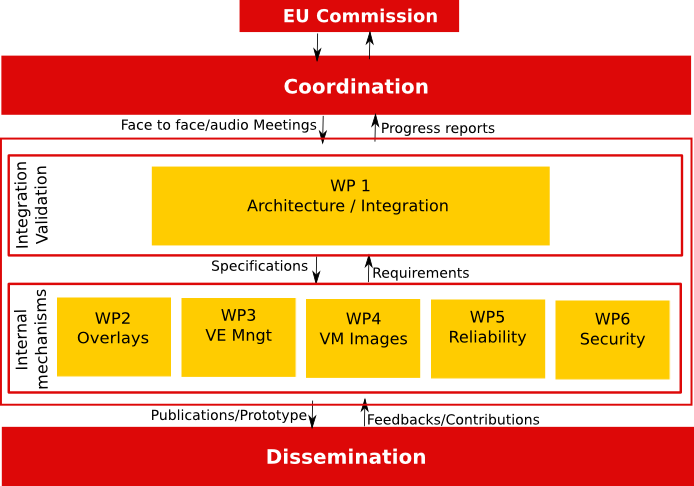
\includegraphics[width=.8\linewidth]{FIGS/pert-4.png}
\caption{Work Package Organization}
\label{fig:wp-org}
\end{center}
\end{figure}

\subsection{Consortium as a Whole}
Currently, the DISCOVERY consortium is composed of 3 research group,  Inria (France), the storage research group from BSC (Spain),and the CRS4 in Sardinia. Three European NRENs and one telco complete the consortium: RENATER (French NREN), PSNC (Polish NREN), GRNET (Greek NREN) and Orange Labs (France). This geographic
pluralism coupled with the privileged relationships the participants in the
project enjoy with the different communities guarantee a wide
dissemination of the \discovery results.

From the scientific point of view, the consortium gathers the expertise of
well-recognized research groups dealing for several years with
Cluster/Grid/Cloud/P2P Computing challenges. By integrating important and well-established network operators, 
we point out that the consortium has the complete knowledge necessary to reach the objectives of DISCOVERY project.
This association of strong research groups and major network partners assures prime scientific
results to the DISCOVERY project while securing a wide possible exploitation impact. 

Finally, it is worth nothing that most of the members are used to collaborate
directly around formal or informal collaborations. 
%
From the industrial point of view, Inria and Orange Labs have been
collaborating for several years around different projects such as ANR Selfware, ANR SelfXL and
more recently the OpenCloudware FSN project. Regarding RENATER, several members
of the consortium are used to interact with the main technical leaders through
the Grid'5000 project. 
%
At the European level,  ASCOLA and BSC have been taking part the European Marie Curie Initial Training Network
SCALUS, SCALing by means of Ubiquitous Storage since 2009. In (Lèbre, et al.
March 2011), ASCOLA with CRS4 conducted a prospective study that sketch out the
premises of the current DISCOVERY proposal.  
All these fruitful collaborations are
excellent indicators for the successfully achievement of the DISCOVERY project. 

%
%\smallskip\noindent\begin{xtabular}{|p{12mm}|p{122mm}|p{23mm}|}
%T0+12 & First year progress report & \ALinst  \\\hline
%\multicolumn{1}{|c}{} & \multicolumn{2}{p{145mm}|}{
% Presentation of the \discovery architecture overview, the APIs and  its internals }\\\hline
%T0+12 & First \textit{Proof-of-Concept}  & \ALinst \\\hline
%\multicolumn{1}{|c}{} & \multicolumn{2}{p{145mm}|}{
%  First Proof-of-Concept, integrating the first mechanisms 
%that enable to start a VE from any peers of the infrastructure according to the resource availability and the expectations of the VE.
%}\\\hline
%T0+24 & Final progress report & \ALinst  \\\hline
%\multicolumn{1}{|c}{} & \multicolumn{2}{p{145mm}|}{
%	Final document presentating the complete \discovery architecture, the APIs between the different internal components
%and detailing the scientific results.}\\\hline 
%T0+24 & Release of an alpha version of the \discovery system & \ \\\hline
%\multicolumn{1}{|c}{} & \multicolumn{2}{p{145mm}|}{
%  Release of a alpha version of the \discovery system integrating each mechanism designed and implemented in other tasks.
%}\\\hline
%\end{xtabular}
%
%\subsubsection{Dissemination and Exploitation of Results}
%Some of the partners are used to formal collaborations through recent
%projects. The obtained results will be published as research reports, as well
%as in the proceedings of conferences and in journals. Code developed in this
%project will remain the property of the employers of the members developing
%them. It will be distributed under the ``GNU Lesser General Public License''
%(LGPL), which is compatible both with free licenses such as the GNU GPL license
%while allowing to use proprietary softwares. 
%
%To increase the visibility of the \discovery initiative, a first action
%consists in promoting the LUC idea at international conferences either by
%presenting direct results of the different WPs or by giving more general talks
%as invited speaker in colocated workshops. The members of the consortium are
%involved in different program committees of conferences or workshops. The
%strong involvement of each member in their community will be a significant
%advantage to promote the \discovery idea.  
%We also plan to attend one or two big events such as SuperComputing conferences
%as virtualization becomes also a key item in this extreme-scale infrastructure.
%These events are usually wider than academic conferences, which will enable to
%present the \discovery idea to industrials leading the market of current UC solutions. 
% 
%
%A second action will consist in giving access to the code of the system. A GIT
%repository will be available, delivering an access to the source code and the
%different binaries/documentations of the prototype. The objective is the
%creation of a \discovery community where everyone will be able to contribute to
%the \discovery system either by stabilizing the code or by extending it with
%additional mechanisms. We learned by experience that this model needs important
%efforts of animation for the leaders of the project as  potential contributors
%first have to know about \discovery, then find the project web site or read a
%paper about the system itself to finally contribute to the code.  However, all
%members of the \discovery initiative understand the importance of promoting the
%LUC idea and starting to build a community of users and developers of the \discovery
%system before the end of the project. 
 
% Justification of scientific expenses ? 

\bibliographystyle{alpha}
\bibliography{short-proposal}
\end{document}
